\section{Conception de la base de données}

\subsection{Présentation}

La base de données utilisée est \texttt{miniproject\_version\_alpha}. Elle contient sept tables principales : \texttt{fournisseur}, \texttt{client}, \texttt{tarif}, \texttt{consommation}, \texttt{photo\_capteur}, \texttt{anomalie} et \texttt{facture}. Le modèle complet est présenté sur la figure~\ref{fig:msd}.

\begin{figure}[htbp]
  \centering
  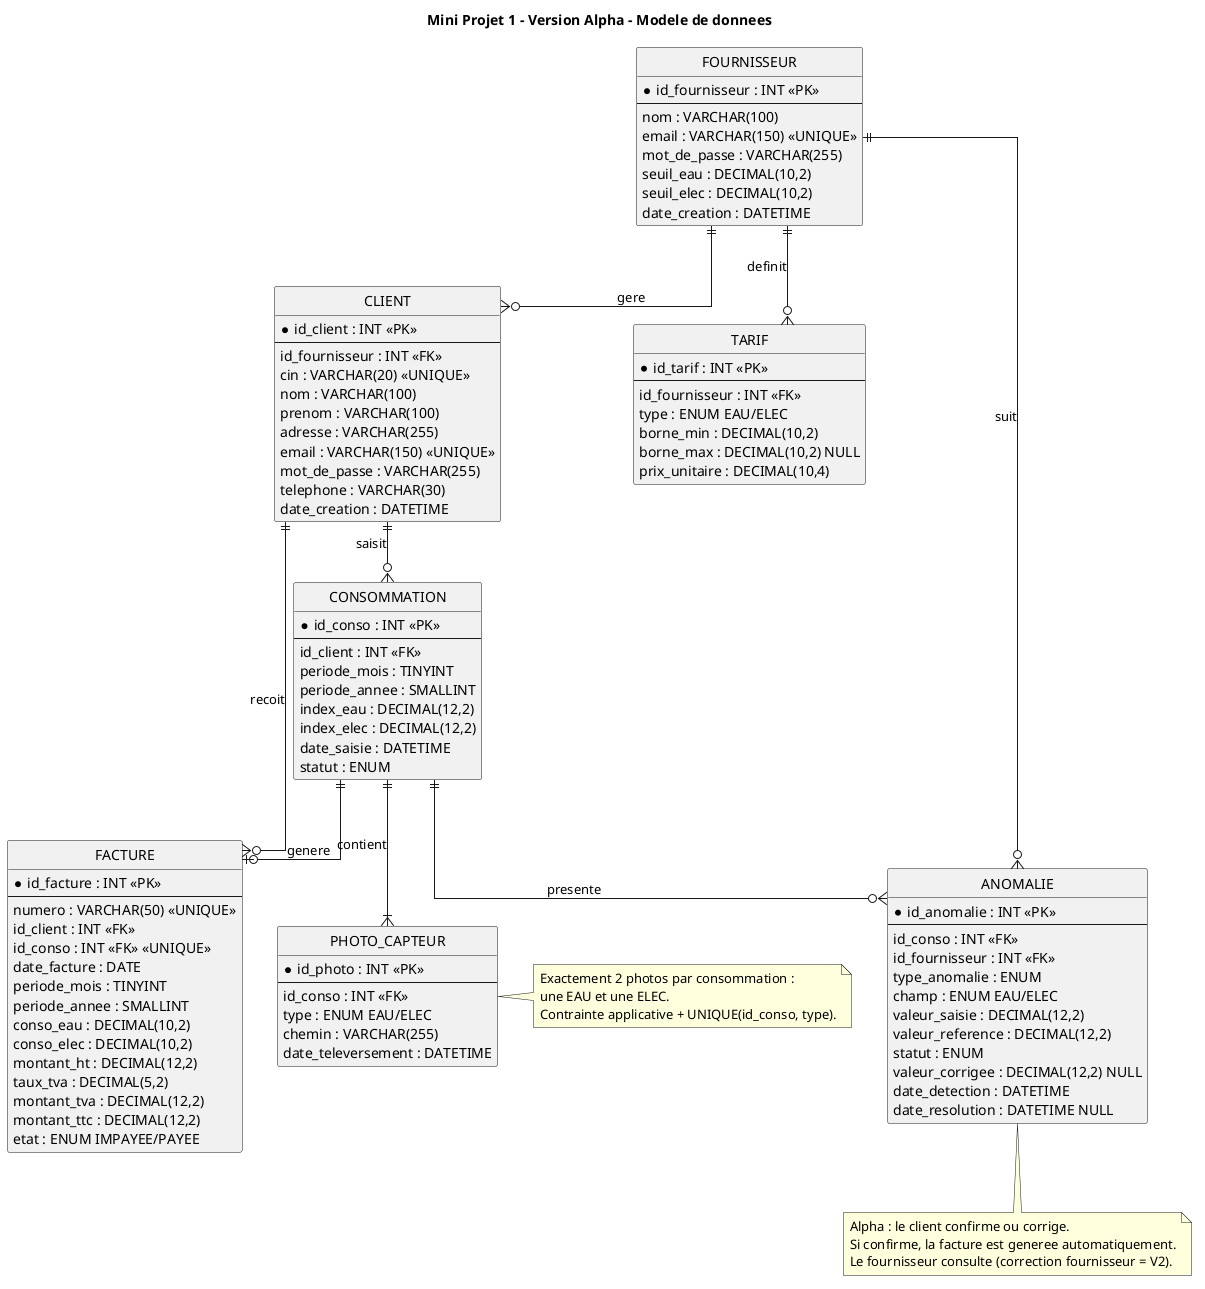
\includegraphics[width=0.85\textwidth]{../conception/msd/msd.png}
  \caption{Modèle de données de la version Alpha}
  \label{fig:msd}
\end{figure}

\subsection{Description des tables}

\begin{longtable}{p{0.20\textwidth}p{0.72\textwidth}}
\caption{Rôle des tables de la base de données}\label{tab:tables}\\
\toprule
\textbf{Table} & \textbf{Description} \\
\midrule
\endfirsthead
\toprule
\textbf{Table} & \textbf{Description} \\
\midrule
\endhead
\texttt{fournisseur} & Informations du fournisseur, identifiants de connexion et seuils de vigilance pour l'eau et l'électricité. \\
\texttt{client} & Informations personnelles, CIN, adresse, email, mot de passe et fournisseur associé. \\
\texttt{tarif} & Tranches tarifaires de l'eau et de l'électricité, avec bornes et prix unitaire. \\
\texttt{consommation} & Index mensuels, période, date de saisie et état du relevé. \\
\texttt{photo\_capteur} & Chemins des photos EAU et ELEC associées à une consommation. \\
\texttt{anomalie} & Type d'anomalie, champ concerné, valeurs de saisie et de référence, état et correction. \\
\texttt{facture} & Numéro, période, consommations, montants HT/TVA/TTC et état de la facture. \\
\bottomrule
\end{longtable}

\subsection{Relations et cardinalités}

\begin{table}[H]
\centering
\caption{Relations principales du modèle}
\label{tab:relations}
\small
\begin{tabular}{p{0.32\textwidth}p{0.18\textwidth}p{0.38\textwidth}}
\toprule
\textbf{Relation} & \textbf{Cardinalité} & \textbf{Implémentation} \\
\midrule
Fournisseur -- Client & 1..1 -- 0..n & \texttt{client.id\_fournisseur} \\
Fournisseur -- Tarif & 1..1 -- 0..n & \texttt{tarif.id\_fournisseur} \\
Fournisseur -- Anomalie & 1..1 -- 0..n & \texttt{anomalie.id\_fournisseur} \\
Client -- Consommation & 1..1 -- 0..n & \texttt{consommation.id\_client} \\
Client -- Facture & 1..1 -- 0..n & \texttt{facture.id\_client} \\
Consommation -- Anomalie & 1..1 -- 0..n & \texttt{anomalie.id\_conso} \\
Consommation -- Facture & 1..1 -- 0..1 & \texttt{facture.id\_conso} UNIQUE \\
Consommation -- Photo & 1..1 -- 2..2 & \texttt{photo\_capteur.id\_conso}\newline UNIQUE(\texttt{id\_conso},\texttt{type}) \\
\bottomrule
\end{tabular}
\end{table}

La version Alpha utilise un fournisseur unique. La colonne \texttt{id\_fournisseur} est néanmoins conservée dans les tables \texttt{client}, \texttt{tarif} et \texttt{anomalie} pour préserver l'intégrité référentielle et permettre une évolution vers plusieurs fournisseurs.

\subsection{Intégrité et contraintes}

\begin{itemize}[leftmargin=*]
  \item moteur \textbf{InnoDB} et encodage \texttt{utf8mb4} ;
  \item clés étrangères avec \texttt{ON DELETE RESTRICT} pour les données maîtres ;
  \item \texttt{ON DELETE CASCADE} pour les photos et anomalies liées à une consommation ;
  \item unicité du CIN et de l'email du client ;
  \item unicité de l'email du fournisseur ;
  \item unicité de la période de consommation par client : \texttt{(id\_client, periode\_mois, periode\_annee)} ;
  \item unicité du type de photo par consommation : \texttt{(id\_conso, type)} ;
  \item unicité du numéro de facture et de la consommation facturée ;
  \item contraintes de vérification sur les index, les montants et les bornes tarifaires.
\end{itemize}

\subsection{États et tarifs}

\begin{table}[H]
\centering
\caption{États utilisés dans la base}
\label{tab:etats}
\small
\begin{tabular}{p{0.20\textwidth}p{0.65\textwidth}}
\toprule
\textbf{Table} & \textbf{États} \\
\midrule
\texttt{consommation} & \texttt{EN\_ATTENTE}, \texttt{ANOMALIE}, \texttt{VALIDEE}, \texttt{FACTUREE} \\
\texttt{anomalie} & \texttt{EN\_ATTENTE}, \texttt{CONFIRMEE}, \texttt{CORRIGEE} \\
\texttt{facture} & \texttt{IMPAYEE}, \texttt{PAYEE} \\
\bottomrule
\end{tabular}
\end{table}

\begin{table}[H]
\centering
\caption{Tranches tarifaires appliquées}
\label{tab:tarifs}
\small
\begin{tabular}{p{0.12\textwidth}p{0.20\textwidth}p{0.20\textwidth}p{0.20\textwidth}}
\toprule
\textbf{Type} & \textbf{Tranche 1} & \textbf{Tranche 2} & \textbf{Tranche 3+} \\
\midrule
Eau & 0--6 m\textsuperscript{3} : 2,37 DH & 6--20 m\textsuperscript{3} : 7,39 DH & 20--35 : 10,98 DH ; >35 : 11,03 DH \\
Électricité & 0--100 kWh : 0,82 DH & 100--150 kWh : 0,92 DH & >150 kWh : 1,10 DH \\
\bottomrule
\end{tabular}
\end{table}

La TVA appliquée est de 18 \%. Les montants sont arrondis à deux décimales.

\subsection{Jeu de données de démonstration}

Le script \texttt{sql/seed.sql} insère un fournisseur, trois clients, sept tarifs et une consommation de septembre 2026 pour chaque client. Ce jeu de données permet de tester la saisie du mois suivant, l'affichage du relevé précédent et la génération des factures.
